\documentclass[aspectratio=169,11pt]{beamer}

\usepackage[T1]{fontenc}
\usepackage{tikz}
\usetikzlibrary{arrows.meta,positioning}

% A small, dependency-light visual system intended to compile with a standard
% TeX Live installation that includes Beamer and PGF/TikZ.
\definecolor{RlmNavy}{HTML}{17324D}
\definecolor{RlmTeal}{HTML}{168A83}
\definecolor{RlmGold}{HTML}{D49A2A}
\definecolor{RlmRed}{HTML}{B34C4C}
\definecolor{RlmInk}{HTML}{263238}
\definecolor{RlmMuted}{HTML}{65757F}
\definecolor{RlmPaper}{HTML}{F7F9FA}

\setbeamercolor{normal text}{fg=RlmInk,bg=white}
\setbeamercolor{structure}{fg=RlmNavy}
\setbeamercolor{frametitle}{fg=RlmNavy,bg=white}
\setbeamercolor{alerted text}{fg=RlmRed}
\setbeamercolor{block title}{fg=white,bg=RlmNavy}
\setbeamercolor{block body}{fg=RlmInk,bg=RlmPaper}
\setbeamercolor{block title alerted}{fg=white,bg=RlmRed}
\setbeamercolor{block body alerted}{fg=RlmInk,bg=RlmRed!7}
\setbeamercolor{author in head/foot}{fg=RlmMuted,bg=white}
\setbeamercolor{date in head/foot}{fg=RlmMuted,bg=white}

\setbeamertemplate{navigation symbols}{}
\setbeamertemplate{blocks}[rounded][shadow=false]
\setbeamertemplate{itemize item}{\color{RlmTeal}\small$\blacktriangleright$}
\setbeamertemplate{itemize subitem}{\color{RlmTeal}\scriptsize$\bullet$}
\setbeamertemplate{footline}{%
  \leavevmode%
  \hbox{%
    \begin{beamercolorbox}[wd=.84\paperwidth,ht=2.7ex,dp=1.1ex,leftskip=.55cm]{author in head/foot}%
      Preliminary and exploratory research
    \end{beamercolorbox}%
    \begin{beamercolorbox}[wd=.16\paperwidth,ht=2.7ex,dp=1.1ex,rightskip=.55cm plus 1fil]{date in head/foot}%
      \hfill\insertframenumber/\inserttotalframenumber
    \end{beamercolorbox}%
  }%
}

\setbeamerfont{title}{size=\LARGE,series=\bfseries}
\setbeamerfont{subtitle}{size=\large}
\setbeamerfont{frametitle}{size=\Large,series=\bfseries}

\tikzset{
  rlmstage/.style={
    draw=RlmNavy!28,
    fill=RlmPaper,
    rounded corners=3pt,
    minimum height=1.1cm,
    align=center,
    inner sep=6pt
  },
  rlmfocus/.style={
    rlmstage,
    draw=RlmTeal,
    fill=RlmTeal!9
  },
  rlmarrow/.style={-{Latex[length=2.3mm]},thick,draw=RlmTeal}
}

\begin{document}

% Slide 1 -------------------------------------------------------------------
\begin{frame}[plain]
  \vspace{0.4cm}
  {\usebeamerfont{title}\color{RlmNavy}
    Can a model build an unfamiliar solution from familiar pieces?\par}

  \vspace{0.25cm}
  {\usebeamerfont{subtitle}\color{RlmMuted}
    Preliminary and exploratory research update\par}

  \vspace{0.65cm}
  \begin{beamercolorbox}[wd=\linewidth,sep=1em,rounded=true]{block body}
    \centering
    \Large
    Language models are strongest when a problem resembles something they have seen before.\\[0.45em]
    We are studying whether a Recursive Language Model (RLM) can turn a new, difficult problem
    into \textbf{smaller, more familiar problems}.
  \end{beamercolorbox}

  \vfill
  \begin{columns}[T,onlytextwidth]
    \begin{column}{0.48\textwidth}
      \centering
      {\color{RlmTeal}\textbf{We completed several preliminary training studies.}}\\[0.25em]
      The model learned several ways to work inside the RLM.
    \end{column}
    \begin{column}{0.48\textwidth}
      \centering
      {\color{RlmGold}\textbf{The larger question remains open.}}\\[0.25em]
      Can this process help on genuinely new problems?
    \end{column}
  \end{columns}

  \vspace{0.35cm}
  {\small\color{RlmMuted}Research discussion \hfill 29 August 2026}
\end{frame}

% Slide 2 -------------------------------------------------------------------
\begin{frame}{An RLM gives the model a workspace and a way to hand off work.}
  \centering
  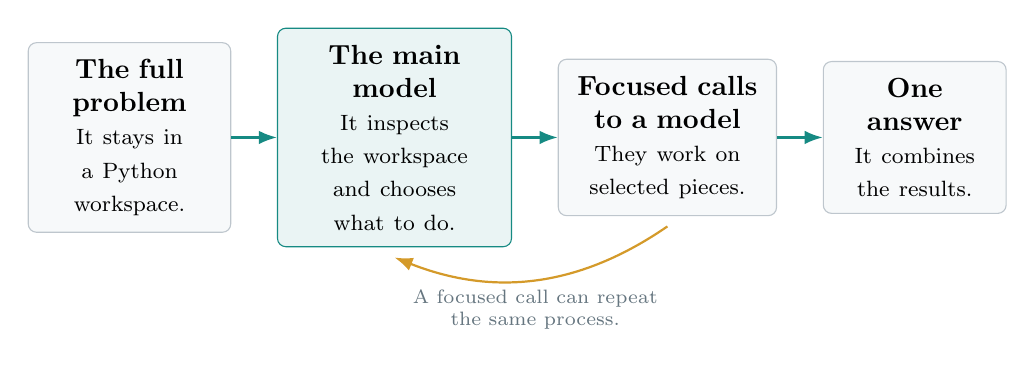
\begin{tikzpicture}[node distance=.58cm]
    \node[rlmstage,text width=2.15cm] (workspace) {
      \textbf{The full problem}\\
      \footnotesize It stays in a Python workspace.
    };
    \node[rlmfocus,right=of workspace,text width=2.55cm] (root) {
      \textbf{The main model}\\
      \footnotesize It inspects the workspace and chooses what to do.
    };
    \node[rlmstage,right=of root,text width=2.35cm] (calls) {
      \textbf{Focused calls to a model}\\
      \footnotesize They work on selected pieces.
    };
    \node[rlmstage,right=of calls,text width=1.9cm] (answer) {
      \textbf{One answer}\\
      \footnotesize It combines the results.
    };
    \draw[rlmarrow] (workspace) -- (root);
    \draw[rlmarrow] (root) -- (calls);
    \draw[rlmarrow] (calls) -- (answer);
    \draw[-{Latex[length=2.3mm]},thick,draw=RlmGold]
      ([yshift=-.13cm]calls.south) to[bend left=28]
      node[below,align=center,font=\scriptsize,text=RlmMuted]
      {A focused call can repeat\\
      the same process.}
      ([yshift=-.13cm]root.south);
  \end{tikzpicture}

  \vspace{0.65cm}
  \begin{block}{The main model may never need to read the entire original input at once.}
    It can use code to inspect selected parts, ask other model calls to work on those parts, and
    combine the returned results. The Python workspace holds the large input and the intermediate
    work.
  \end{block}

  \vspace{0.1cm}
  {\small\color{RlmMuted}
    The RLM supplies the workspace and lets focused model calls repeat the same process. The main
    model still decides what to inspect, how to divide the work, and when it has enough evidence
    to answer.}
\end{frame}

% Slide 3 -------------------------------------------------------------------
\begin{frame}{The larger idea: solve a new whole by combining familiar pieces.}
  \centering
  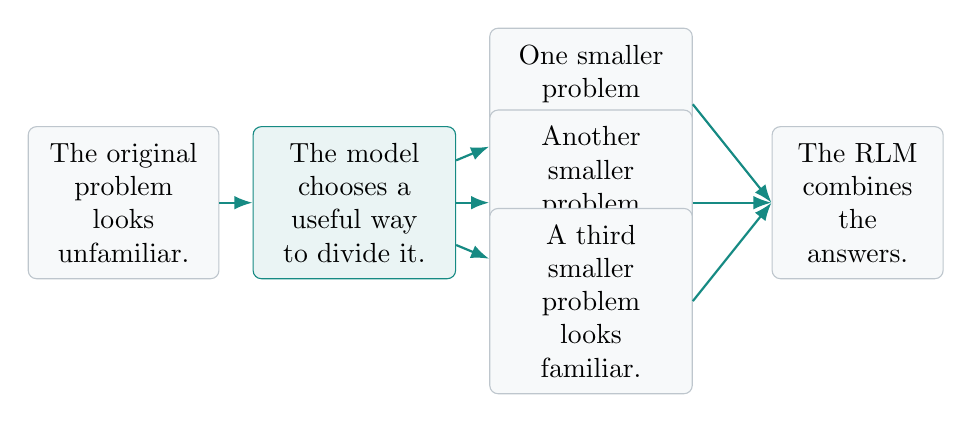
\begin{tikzpicture}[node distance=.42cm]
    \node[rlmstage,text width=2.0cm] (new) {The original problem looks unfamiliar.};
    \node[rlmfocus,right=of new,text width=2.15cm] (split) {The model chooses a useful way to divide it.};
    \node[rlmstage,right=of split,yshift=1.25cm,text width=2.15cm] (a) {One smaller problem looks familiar.};
    \node[rlmstage,right=of split,text width=2.15cm] (b) {Another smaller problem looks familiar.};
    \node[rlmstage,right=of split,yshift=-1.25cm,text width=2.15cm] (c) {A third smaller problem looks familiar.};
    \node[rlmstage,right=1.0cm of b,text width=1.75cm] (combine) {The RLM combines the answers.};
    \draw[rlmarrow] (new) -- (split);
    \draw[rlmarrow] (split) -- (a);
    \draw[rlmarrow] (split) -- (b);
    \draw[rlmarrow] (split) -- (c);
    \draw[rlmarrow] (a.east) -- (combine.west);
    \draw[rlmarrow] (b.east) -- (combine.west);
    \draw[rlmarrow] (c.east) -- (combine.west);
  \end{tikzpicture}

  \vspace{0.3cm}
  \begin{block}{Researchers call this compositional generalization.}
    Each model call may only need to solve a local problem that resembles its training experience.
    The RLM keeps track of the work, sends the pieces to focused model calls, and brings the
    answers together. In this way, the system may solve a new whole by combining familiar parts.
  \end{block}

  \vspace{0.12cm}
  {\small\color{RlmMuted}
    Our research asks when this division works, where it fails, and whether training can improve
    the choices that the model makes.}

  \vfill
  {\tiny\color{RlmMuted}
    These ideas are motivated by \href{https://alexzhang13.github.io/blog/2025/rlm/}{Alex Zhang,
    ``Recursive Language Models''} and
    \href{https://alexzhang13.github.io/blog/2026/harness/}{``Harnesses are compositional
    generalizers.''}}
\end{frame}

% Slide 4 -------------------------------------------------------------------
\begin{frame}{We can now repeat the full supervised train-and-test process.}
  \begin{beamercolorbox}[wd=\linewidth,sep=.75em,rounded=true]{block body}
    \textbf{Supervised fine-tuning (SFT)} means showing the model good worked examples and
    training it to imitate the useful decisions in those examples.
  \end{beamercolorbox}

  \vspace{0.5cm}
  \centering
  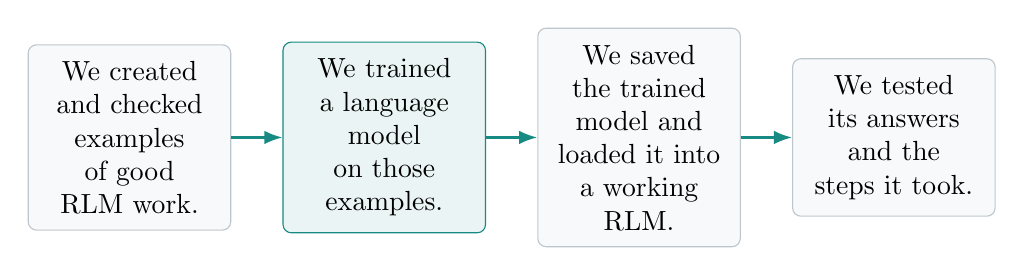
\begin{tikzpicture}[node distance=.65cm]
    \node[rlmstage,text width=2.15cm] (examples) {We created and checked examples of good RLM work.};
    \node[rlmfocus,right=of examples,text width=2.15cm] (train) {We trained a language model on those examples.};
    \node[rlmstage,right=of train,text width=2.15cm] (reload) {We saved the trained model and loaded it into a working RLM.};
    \node[rlmstage,right=of reload,text width=2.15cm] (evaluate) {We tested its answers and the steps it took.};
    \draw[rlmarrow] (examples) -- (train);
    \draw[rlmarrow] (train) -- (reload);
    \draw[rlmarrow] (reload) -- (evaluate);
  \end{tikzpicture}

  \vspace{0.55cm}
  \begin{block}{The complete training loop now works across successive studies.}
    We can train a model, save intermediate versions, put a chosen version back inside the RLM,
    and evaluate it on examples that were not used for training.
  \end{block}

  \vspace{0.1cm}
  {\small\color{RlmMuted}
    This turns the idea into a repeatable experiment: we can compare training methods and test
    whether improvements carry over to genuinely new tasks.}
\end{frame}

% Slide 5 -------------------------------------------------------------------
\begin{frame}{Training taught the model to use the RLM on controlled tasks.}
  \centering
  {\small\color{RlmMuted}New test tasks solved before and after supervised training}

  \vspace{0.35cm}
  \begin{columns}[T,onlytextwidth]
    \begin{column}{0.48\textwidth}
      \centering
      \textbf{Inspect, then calculate}

      \vspace{0.25cm}
      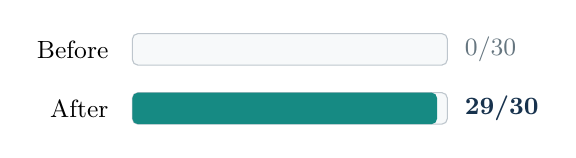
\begin{tikzpicture}
        \node[anchor=east,font=\small] at (0,1.18) {Before};
        \draw[rounded corners=2pt,draw=RlmNavy!28,fill=RlmPaper]
          (0.18,.98) rectangle (4.18,1.38);
        \node[anchor=west,font=\small,text=RlmMuted] at (4.28,1.18) {0/30};

        \node[anchor=east,font=\small] at (0,.43) {After};
        \draw[rounded corners=2pt,draw=RlmNavy!28,fill=RlmPaper]
          (0.18,.23) rectangle (4.18,.63);
        \fill[rounded corners=2pt,RlmTeal]
          (0.18,.23) rectangle (4.05,.63);
        \node[anchor=west,font=\small,text=RlmNavy] at (4.28,.43) {\textbf{29/30}};
      \end{tikzpicture}

      {\small The model learned a simple two-step routine.}
    \end{column}

    \begin{column}{0.48\textwidth}
      \centering
      \textbf{Use one program for six operations}

      \vspace{0.25cm}
      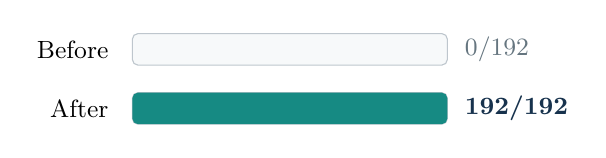
\begin{tikzpicture}
        \node[anchor=east,font=\small] at (0,1.18) {Before};
        \draw[rounded corners=2pt,draw=RlmNavy!28,fill=RlmPaper]
          (0.18,.98) rectangle (4.18,1.38);
        \node[anchor=west,font=\small,text=RlmMuted] at (4.28,1.18) {0/192};

        \node[anchor=east,font=\small] at (0,.43) {After};
        \draw[rounded corners=2pt,draw=RlmNavy!28,fill=RlmPaper]
          (0.18,.23) rectangle (4.18,.63);
        \fill[rounded corners=2pt,RlmTeal]
          (0.18,.23) rectangle (4.18,.63);
        \node[anchor=west,font=\small,text=RlmNavy] at (4.28,.43) {\textbf{192/192}};
      \end{tikzpicture}

      {\small The model learned a reusable but narrow mechanism.}
    \end{column}
  \end{columns}

  \vspace{0.5cm}
  \begin{block}{The change was large and repeatable within these small, controlled tests.}
    Before training, the model did not reliably perform either RLM routine. After training, it
    performed them on almost every new test task.
  \end{block}

  \vspace{0.08cm}
  {\scriptsize\color{RlmMuted}
    This establishes that training can change how the model uses the RLM. It does not yet show
    broad problem-solving or reliable handoffs to other model calls.}
\end{frame}

% Slide 6 -------------------------------------------------------------------
\begin{frame}{The model learned step-by-step work before reliable handoffs.}
  \begin{columns}[T,onlytextwidth]
    \begin{column}{0.57\textwidth}
      \centering
      \textbf{What the model learned in a small test}

      \vspace{0.28cm}
      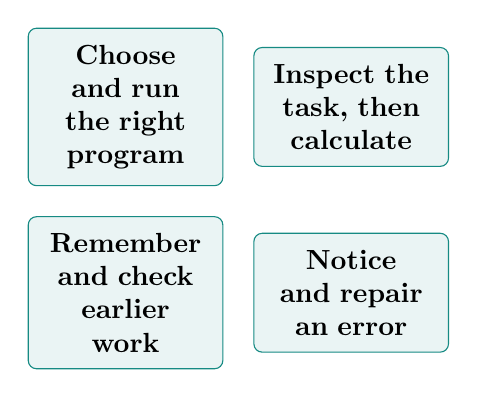
\begin{tikzpicture}[node distance=.38cm]
        \node[rlmfocus,text width=2.05cm] (choose) {\textbf{Choose and run the right program}};
        \node[rlmfocus,right=of choose,text width=2.05cm] (inspect) {\textbf{Inspect the task, then calculate}};
        \node[rlmfocus,below=of choose,text width=2.05cm] (remember) {\textbf{Remember and check earlier work}};
        \node[rlmfocus,right=of remember,text width=2.05cm] (repair) {\textbf{Notice and repair an error}};
      \end{tikzpicture}

      \vspace{0.25cm}
      {\small The model solved \textbf{24 of 36 tasks overall}: every task across these four
      kinds of step-by-step work.}
    \end{column}

    \begin{column}{0.39\textwidth}
      \centering
      \textbf{The key next capability}

      \vspace{0.28cm}
      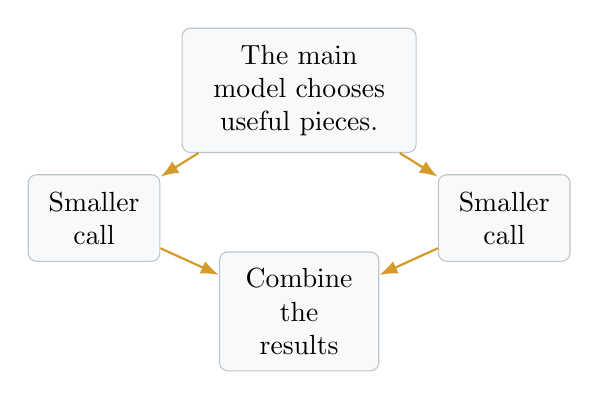
\begin{tikzpicture}[node distance=.38cm]
        \node[rlmstage,text width=2.55cm] (main) {The main model chooses useful pieces.};
        \node[rlmstage,below left=of main,text width=1.25cm] (a) {Smaller\\call};
        \node[rlmstage,below right=of main,text width=1.25cm] (b) {Smaller\\call};
        \node[rlmstage,below=1.25cm of main,text width=1.6cm] (combine) {Combine the results};
        \draw[-{Latex[length=2.3mm]},thick,draw=RlmGold] (main) -- (a);
        \draw[-{Latex[length=2.3mm]},thick,draw=RlmGold] (main) -- (b);
        \draw[-{Latex[length=2.3mm]},thick,draw=RlmGold] (a) -- (combine);
        \draw[-{Latex[length=2.3mm]},thick,draw=RlmGold] (b) -- (combine);
      \end{tikzpicture}

      \vspace{0.25cm}
      {\small It did not solve the \textbf{12 tasks} that required model-to-model handoffs.
      Learning those handoffs is the bridge to the larger RLM idea.}
    \end{column}
  \end{columns}

  \vspace{0.4cm}
  \begin{beamercolorbox}[wd=\linewidth,sep=.6em,rounded=true]{block body}
    \centering
    The current evidence supports learned \textbf{step-by-step work inside the workspace}. It
    does not yet establish the full idea of repeatedly dividing a problem among model calls.
  \end{beamercolorbox}
\end{frame}

% Slide 7 -------------------------------------------------------------------
\begin{frame}{Next, we will test learning from successful attempts inside the RLM.}
  \begin{beamercolorbox}[wd=\linewidth,sep=.55em,center,rounded=true]{block body alerted}
    \textbf{We have designed this experiment, but we have not run it yet.}
  \end{beamercolorbox}

  \vspace{0.4cm}
  \centering
  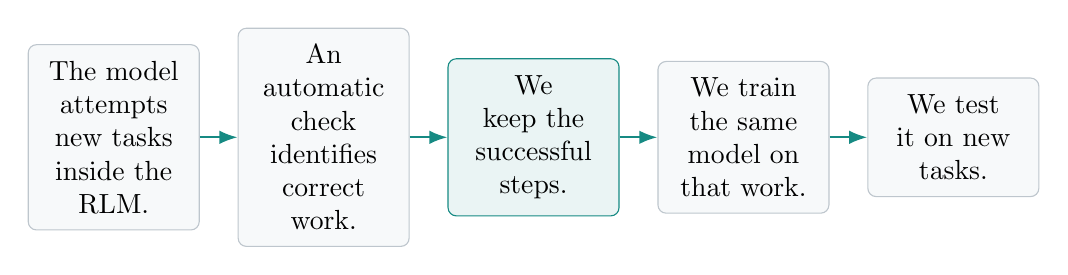
\begin{tikzpicture}[node distance=.48cm]
    \node[rlmstage,text width=1.75cm] (attempt) {The model attempts new tasks inside the RLM.};
    \node[rlmstage,right=of attempt,text width=1.75cm] (check) {An automatic check identifies correct work.};
    \node[rlmfocus,right=of check,text width=1.75cm] (keep) {We keep the successful steps.};
    \node[rlmstage,right=of keep,text width=1.75cm] (train) {We train the same model on that work.};
    \node[rlmstage,right=of train,text width=1.75cm] (test) {We test it on new tasks.};
    \draw[rlmarrow] (attempt) -- (check);
    \draw[rlmarrow] (check) -- (keep);
    \draw[rlmarrow] (keep) -- (train);
    \draw[rlmarrow] (train) -- (test);
  \end{tikzpicture}

  \vspace{0.45cm}
  \begin{block}{The comparison is designed to answer a simple question.}
    Does practice inside the RLM teach something beyond ordinary task practice? We will compare a
    model trained on direct solutions with a model trained on successful RLM work.
  \end{block}

  \vspace{0.12cm}
  {\small\color{RlmMuted}
    When an answer is wrong, we will ask whether the model divided the problem poorly, solved a
    piece incorrectly, or combined the pieces incorrectly. This makes failures more informative.}

  \vfill
\end{frame}

% Slide 8 -------------------------------------------------------------------
\begin{frame}{The next experiments will test the larger idea directly.}
  \begin{columns}[T,onlytextwidth]
    \begin{column}{0.31\textwidth}
      \begin{block}{First, we will test whether learning carries over.}
        We will ask whether learning carries to new examples, new formats, and eventually new kinds
        of problems.
      \end{block}
    \end{column}
    \begin{column}{0.31\textwidth}
      \begin{block}{Then, we will ask what caused any improvement.}
        We will compare useful ways of dividing the problem with ordinary practice and with simply
        giving the model more calls.
      \end{block}
    \end{column}
    \begin{column}{0.31\textwidth}
      \begin{block}{Later, the model may learn from scores.}
        Once scores reliably separate good and bad attempts, reward-based training can improve the
        model's decisions.
      \end{block}
    \end{column}
  \end{columns}

  \vspace{0.55cm}
  \begin{beamercolorbox}[wd=\linewidth,sep=1em,rounded=true]{block body}
    \centering
    \large
    \textbf{The big picture}\par
    \vspace{0.35em}
    We are testing whether training a model to use the RLM can help it solve unfamiliar
    problems by building solutions from familiar pieces.
  \end{beamercolorbox}

  \vfill
  \centering
  {\color{RlmTeal}\textbf{We would value suggestions about good test problems, fair comparisons,
  and risks that we may be overlooking.}}
\end{frame}

\end{document}
